\documentclass[letterpaper]{article}
\usepackage{natbib,alifexi}
\usepackage[bordercolor=gray!20,backgroundcolor=blue!10,linecolor=blue,textsize=footnotesize,textwidth=0.8in]{todonotes}
\usepackage{hyperref}
\usepackage{algpseudocode}
\usepackage{algorithm}
\usepackage{subfig}

\title{Meta Reinforcement Learning Acrobot}
\author{Florentin Hennecker \\
\mbox{}\\
Universit\'e Libre de Bruxelles, Boulevard du Triomphe - CP 212, 1050
Brussels, Belgium \\
fhenneck@ulb.ac.be}

\marginparwidth=0.5in
\newcommand\Tstrut{\rule{0pt}{2.6ex}}
\newcommand\Bstrut{\rule[-0.9ex]{0pt}{0pt}}


\begin{document}
\maketitle

\begin{abstract}
	Abstract
\end{abstract}

\section{Introduction}
There have been incredible advances in the field of reinforcement learning
in the past few years. Deep Q-learning \citep{dqn, dqn_nature} made learning Atari
games from visual inputs possible, even beating the human level benchmark
for some games; less than two years later, a similar milestone has been reached
for playing Doom, a complex 3D game \citep{doom} using the VizDoom environment
\citep{vizdoom}. Most of these achievements share one issue: once the agents
described in these papers have learned to solve the task they were handed,
they are likely to fail on slightly different versions of the task and will
have to be completely retrained for new tasks, however similar they are from
the task the agent was trained on.

Just like humans use prior knowledge to quickly learn new tasks that are
presented to them, training an agent to learn to solve variations of a problem
is unlikely to be possible without giving it some sort of prior knowledge.
A second key component needed for a fast-learning agent would be a good
learning strategy (\textit{in the sense where $\epsilon$-greedy or softmax selection
\citep{suttonbarto}, Q-learning \citep{qlearning} and SARSA \citep{sarsa} 
are learning strategies})
that takes into account prior knowledge and takes action
to learn about the problem as fast as it can to perform optimally as
soon as possible.

Finding such a strategy is hard, but it can be cast as a reinforcement
learning problem: instead of designing a learning strategy by hand and
teaching the agent to solve a task, \cite{learningtorl}
and \cite{fastrlviaslowrl} propose to
teach an agent to learn to solve a task. The agent presented by Wang et al. is 
an A2C (a single-threaded version of A3C \citep{a3c})
agent with a recurrent connection and presents
two major differences compared to a standard reinforcement learning agent: 
\begin{enumerate}
	\item the agent is trained on trials of episodes rather than on single
		episodes, replicating the training process in standard 
		reinforcement learning
	\item the agent receives process-level information as well as
		an observation of the enviromnent: the reward at the previous
		timestep, the action that led to that reward and an 
		episode termination flag.
\end{enumerate}

Conceptually, in standard reinforcement learning, the network represents 
a policy and its goal is to collect an optimal reward for one episode. In
meta reinforcement learning, the network represents an algorithm which
learns a policy. Its weights, once trained, encode a learning strategy which
decides how to play episodes to maximise reward across multiple episodes.

Both Wang et al. and Duan et al. show convincing learning behaviour from
the meta-learning agent in various types of bandit problems but also
a complex visual navigation task \citep{learningtonavigate}. In both situations, 
the agent deploys a strategy that performs excellent exploration based on its 
prior knowledge of the structure of the task 
and then exploits the knowledge gained during exploration to perform 
optimally for the following episodes. In situations where it is possible, the
agent is able to perform one-shot learning.

We will apply meta reinforcement learning to a new class of problems with
continuous state spaces and a timestep-based-only reward, generating 
a distribution of similar tasks by shuffling randomly the state observation
vector without indicating to the agent which value is which; but also
by permutating the effects of the agent's action.


\subsection{Background} 
A2C

Acrobot

\begin{figure*}[h]
	\centering
	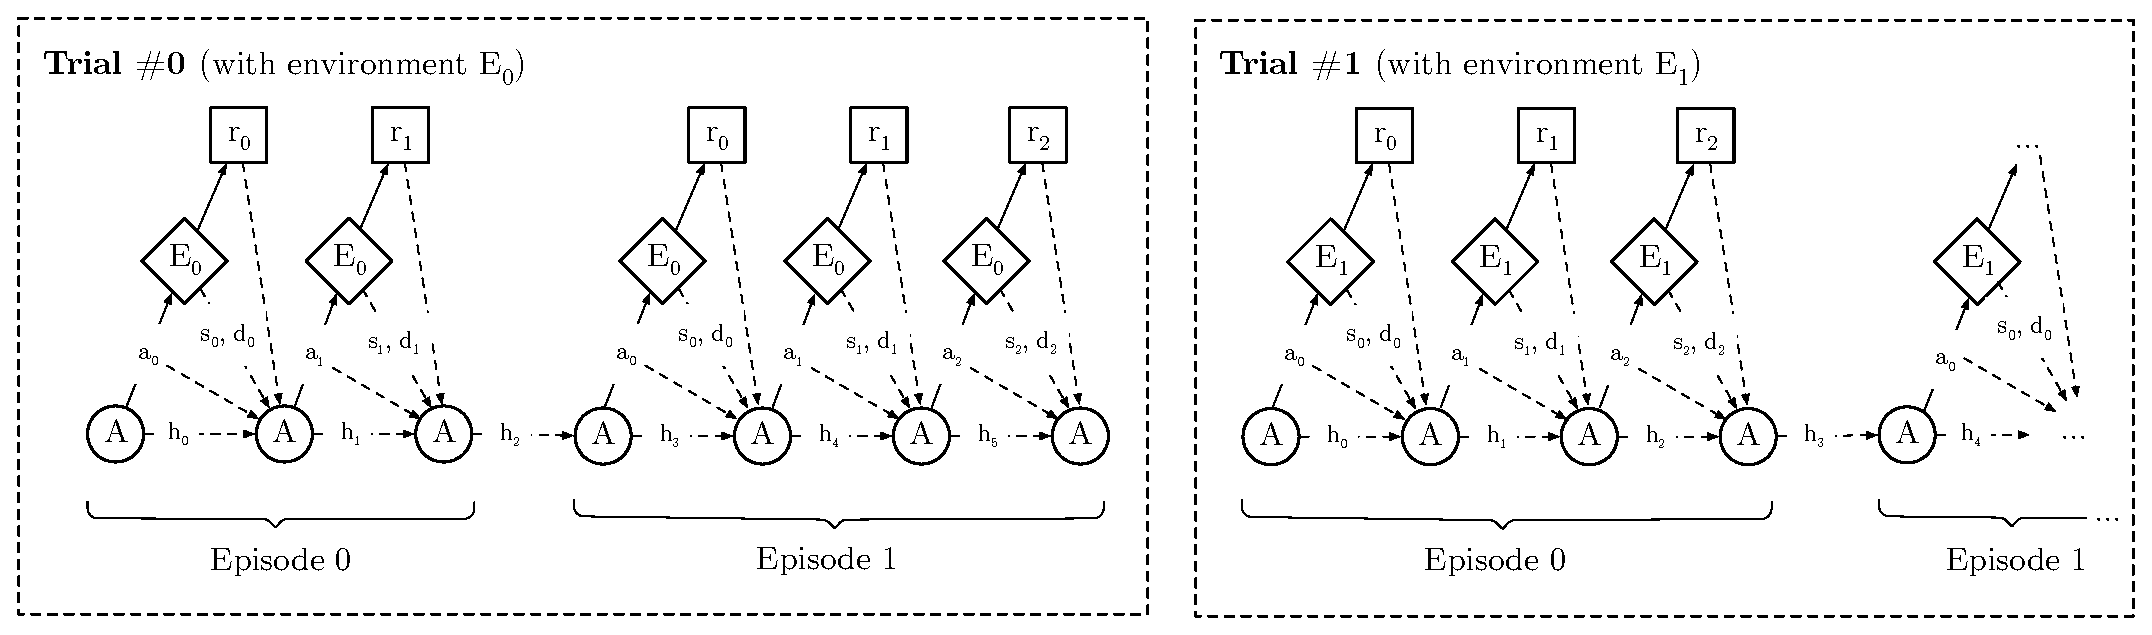
\includegraphics[width=\textwidth]{fig/meta_learning_process.eps}
	\caption{}
	\label{fig:meta_learning_process}
\end{figure*}

\subsection{Model details}

\section{Methods}

\section{Results and discussion}

\section{Conclusions}
\cite{tensorflow}

\footnotesize
\bibliographystyle{apalike}
\bibliography{report}


\end{document}
